% ----------------------------------------------------------
\chapter{Referencial Teórico} \label{cap:referencial}
% ----------------------------------------------------------

\section{Confiabilidade Estrutural}

A confiabilidade pode ser compreendida como a capacidade de um sistema, equipamento, estrutura ou processo de desempenhar suas funções de maneira consistente e previsível, sem apresentar falhas, dentro de um período determinado e sob condições específicas. Em termos práticos, representa o nível de confiança de que um determinado elemento continuará operando conforme esperado, garantindo um desempenho estável ao longo do tempo e diante das variáveis do ambiente em que está inserido \cite{melchers_structural_2017}.

Desse modo, na engenharia estrutural, a confiabilidade é uma disciplina que busca avaliar a probabilidade de uma estrutura manter seu desempenho seguro ao longo de sua vida útil, mesmo considerando incertezas inerentes ao processo. Essas incertezas podem estar associadas a variabilidades nas cargas atuantes, resistência e degradação dos materiais, qualidade da execução e limitações dos modelos de engenharia empregados no dimensionamento e análise da estrutura \cite{melchers_structural_2017, du_structural_2023}.

Essas incertezas podem surgir de fatores como variabilidade nas propriedades dos materiais, condições ambientais, processos construtivos e intensidade de cargas aplicadas. A análise de confiabilidade variante no tempo é uma metodologia adequada para modelar o impacto dessas incertezas sobre o desempenho estrutural ao longo da vida útil de uma estrutura, quantificando os riscos de falha e determinando margens de segurança apropriadas para diferentes condições de exposição e uso \cite{melchers_structural_2017, du_structural_2023, pereira_junior_reliability_2023}.

No estudo da confiabilidade estrutural, a compreensão e quantificação das incertezas são essenciais, dentro das limitações inerentes a cada tipo. As incertezas podem ser classificadas em três categorias: aleatórias (ou intrínsecas), epistêmicas e erro humano. As incertezas epistêmicas decorrem da falta de conhecimento ou de informações insuficientes sobre um determinado fenômeno. À medida que novos dados se tornam disponíveis, esse tipo de incerteza pode ser reduzido ou até eliminado. Exemplos incluem simplificações na modelagem estrutural, aproximações na aplicação de cargas e definição das propriedades dos materiais \cite{du_structural_2023}.

As incertezas aleatórias, por outro lado, são inerentes aos processos físicos envolvidos e não podem ser completamente eliminadas, apenas reduzidas. Entre os principais exemplos, estão as variações naturais das propriedades dos materiais, as oscilações nas condições ambientais e os carregamentos que apresentam comportamento probabilístico. Além disso, o erro humano é um fator que pode influenciar todas as etapas da concepção, execução e manutenção das estruturas, contribuindo para a incerteza global do sistema. A correta identificação e quantificação dessas incertezas são fundamentais para a análise de confiabilidade estrutural, permitindo avaliar os riscos associados ao desempenho da estrutura ao longo de sua vida útil \cite{du_structural_2023}.

Entre os métodos de cálculo da confiabilidade pode-se citar: (\textit{a}) o Método de Primeira Ordem de Confiabilidade (FORM) que utiliza uma linearização da superfície de falha para obter estimativas rápidas e eficientes da probabilidade de falha (Soltani et al., 2021); (\textit{b}) Já o Método de Segunda Ordem de Confiabilidade (SORM) considera a curvatura da superfície de falha, proporcionando estimativas mais precisas; (\textit{c}) Os métodos de amostragem como a Simulação de Monte Carlo é amplamente é utilizada por sua flexibilidade em lidar com modelos complexos, gerando inúmeras amostras aleatórias para modelar o comportamento das variáveis e estimar a probabilidade de falha \cite{pereira_junior_reliability_2023}.

 Para estruturas sujeitas à corrosão, modelos probabilísticos são ferramentas eficazes para integrar variáveis como perda de massa das armaduras, concentração de cloretos e profundidade do cobrimento, fornecendo estimativas precisas das probabilidades de falha e orientando decisões sobre manutenção ou reforço (Vu e Stewart, 2000). A análise probabilística de uma estrutura tem como ponto de partida uma equação conhecida como “Equação de Estado Limite”. Essa equação, expressa por meio da função de estado limite $g(\mathbf{X})$, é uma formulação matemática que descreve o comportamento estrutural com base em critérios de segurança e desempenho estabelecidos para uma determinada condição de uso. De forma geral, essa função pode ser representada conforme a Equação \eqref{eq:g}.

\begin{equation}\label{eq:g}
g(\mathbf{X}) = g(X_1, X_2, X_3, \dots, X_n)
\end{equation} 

A análise da Equação \eqref{eq:g} permite concluir que a falha ocorre quando $g(\textbf{X})\leq0$. Em contraste, quando $g(\textbf{X}) > 0$, a estrutura é considerada segura, pois sua resistência é maior do que as solicitações que atuam sobre ela. Vale ressaltar que a falha nem sempre significa o colapso da estrutura; muitas vezes, ela está relacionada apenas ao não cumprimento de uma verificação específica, definida pela função de falha, onde os valores da variável de solicitação podem ter atingido ou ultrapassado os limites estabelecidos. Quando a Equação de Estado Limite é aplicada no contexto do Estado Limite Último (ELU), ela pode ser interpretada como a margem de segurança da estrutura, conforme expresso na Equação \eqref{eq:g_geral}, em que $\textbf{R}$ representa a resistência da estrutura e $\textbf{S}$ a solicitação atuante.

\begin{equation}\label{eq:g_geral}
g(\mathbf{R}, \mathbf{S}) = \textbf{R} - \textbf{S}
\end{equation} 

Com base nessa Equação de Estado Limite, é possível calcular tanto a probabilidade de falha quanto a de sobrevivência de um elemento estrutural. Conforme explicado por Beck (2019a), a probabilidade de falha de um sistema ou componente estrutural é determinada pela integração da função conjunta de densidade de probabilidade $f_x(\textbf{X})$ no domínio de falha, ou seja, quando $g(\textbf{X})\leq0$, como mostrado na Equação \eqref{eq:pf_geral}.

\begin{equation}\label{eq:pf_geral}
p_f = P[g(\mathbf{X})\leq 0] = \int_{g(\mathbf{X})\leq 0} f_x(\textbf{X}) dx
\end{equation}

% Neste trabalho será adotada a solução por meio de um método de amostragem de Monte Carlo. O modelo parte do pressuposto de gerar um sistema aleatório de partículas com base em uma determinada distribuição de probabilidade. Existem diversas variações do método de Monte Carlo. Neste trabalho, foi utilizado o Monte Carlo com Hipercubo Latino. A estimativa da probabilidade de falha utilizando o método de Monte Carlo é dada pela Equação \eqref{eq:p_f_sum}.

% \begin{equation}
% \label{eq:p_f_sum}
% \hat{p}_f = \frac{1}{n_s} \sum_{i=1}^{n_s} I_f
% \end{equation}

% \begin{equation}
% \label{eq:indicator}
% I_f = 
% \begin{cases}
% 1, & \text{se } g(\mathbf{X}) \leq 0 \\
% 0, & \text{caso contrário}
% \end{cases}
% \end{equation}

% Na Equação \eqref{eq:p_f_sum}, $n_s$ indica o número de amostras. No caso da Equação \eqref{eq:indicator}, o retorno 1 indica falha da função de Estado Limite, ou seja, indica que a estrutura não atendeu a determinado critério, e o retorno 0 indica que a estrutura está na região segura de avaliação da função de Estado Limite. 

% Para calcular o índice de confiabilidade ($\beta$), a Equação \eqref{eq:beta} utiliza a função de distribuição acumulada inversa (CDF) da distribuição normal padrão, denotada como $\Phi^{-1}$.

% \begin{equation}
% \label{eq:beta}
% \beta = -\Phi^{-1}(\hat{p}_f)
% \end{equation}


\section{Método de Amostragem de Monte Carlo com Hipercubo Latino}

Neste estudo, adota-se o método de amostragem de Monte Carlo, cuja origem remonta à década de 1940, quando Ulam e Von Neumann empregaram técnicas probabilísticas para simular fenômenos físicos complexos, especialmente no contexto de cálculos nucleares e aleatórios \cite{ulam_s_monte_1948}. 
Com o avanço da computação, tornou-se uma ferramenta essencial para estimar probabilidades integrando funções de densidades multivariadas, especialmente em contextos onde o cálculo exato é impraticável \cite{song_monte_2023}. 

O modelo parte do pressuposto de gerar um sistema aleatório de partículas com base em uma determinada distribuição de probabilidade. 
Em confiabilidade estrutural, o estimador de falha usual emprega uma função indicadora $I_f$, conforme apresentado na Equação~\eqref{eq:p_f_sum}, onde a probabilidade de falha é estimada por:

\begin{equation}
\label{eq:p_f_sum}
\hat{p}_f = \frac{1}{n_s} \sum_{i=1}^{n_s} I_f
\end{equation}

\begin{equation}
\label{eq:indicator}
I_f =
\begin{cases}
1, & \text{se } g(\mathbf{X}) \leq 0 \\
0, & \text{caso contrário}
\end{cases}
\end{equation}

Na Equação~\eqref{eq:p_f_sum}, $n_s$ indica o número de amostras. 
No caso da Equação~\eqref{eq:indicator}, o retorno $1$ indica falha da função de Estado-Limite, ou seja, que a estrutura não atendeu a determinado critério, e o retorno $0$ indica que a estrutura está na região segura da função de Estado-Limite.

Para calcular o índice de confiabilidade ($\beta$), a Equação~\eqref{eq:beta} utiliza a função de distribuição acumulada inversa (CDF) da distribuição normal padrão, denotada como $\Phi^{-1}$.

\begin{equation}
\label{eq:beta}
\beta = -\Phi^{-1}(\hat{p}_f)
\end{equation}

Existem diversas variações do método de Monte Carlo. Neste trabalho, adotou-se a técnica de Monte Carlo com Hipercubo Latino (\textit{Latin Hypercube Sampling} — LHS), originalmente proposta por \textcite{mckay_comparison_1979} como uma forma de amostragem estratificada voltada à redução da variância das estimativas, quando comparada à amostragem puramente aleatória.

No campo da análise de confiabilidade estrutural, o LHS tem sido amplamente empregado por sua capacidade de aprimorar a eficiência e a representatividade do espaço amostral, assegurando uma distribuição mais uniforme em cada dimensão marginal. Essa característica permite estimar probabilidades de falha com menor número de amostras redundantes, mantendo a precisão dos resultados \cite{helton_latin_2003}.

A utilização do LHS neste estudo tem como objetivo reduzir a variabilidade das estimativas de probabilidade de falha, especialmente em problemas de alta dimensionalidade, proporcionando uma amostragem de boa qualidade sem a necessidade de um número excessivo de simulações \cite{melchers_structural_2017}.

De forma análoga à amostragem estratificada, o método do Hipercubo Latino divide o domínio de cada variável aleatória em intervalos equiprováveis \cite{helton_latin_2003, olsson_latin_2003, helton_signal_2005}. Cada intervalo é amostrado exatamente uma vez, garantindo uma distribuição espaçada e uniforme dos pontos no espaço amostral. Essa propriedade assegura uma cobertura mais homogênea do domínio das variáveis. Um exemplo ilustrativo para o caso bidimensional é apresentado na Figura \ref{fig:lhs}.

\begin{figure}[H]
    \centering
    \caption{Exemplo de correlação entre variáveis no Hipercubo Latino.}
    \label{fig:lhs}
    
\includegraphics[width=0.7\linewidth]{lhs.png}
    \fonte{Autor (2025).}
\end{figure}

Considerando $n$ o número de variáveis aleatórias e $n_s$ o total de amostras geradas, define-se a matriz $P$ de dimensões $(n_s \times n)$, cujas colunas
$P_j = \pi_j(1, 2, \ldots, n_s)$ representam permutações aleatórias da sequência $(1, \ldots, n_s)$, de modo a evitar correlações artificiais entre as variáveis amostradas.
Em seguida, é construída uma matriz $R \in (0,1)_{n_s \times n}$, cujos elementos são mutuamente independentes e seguem uma distribuição uniforme $U(0,1)$ \cite{olsson_latin_2003}.  
Com base nessas duas matrizes, obtém-se a matriz $S$ (Equação \eqref{eq:S_matrix}):

\begin{equation}
S = [s_{ij}]_{n_s \times n} 
= \frac{1}{n_s} (P - R).
\label{eq:S_matrix}
\end{equation}

As amostras normalizadas são então determinadas a partir de $S$ conforme a Equação \eqref{eq:x_samples}:

\begin{equation}
X_j = \{ x_i \}_{i=1,\ldots,n_s} 
= \left\{ F^{-1}_{X_j}(s_{ij}) \right\}_{i=1,\ldots,n_s},
\label{eq:x_samples}
\end{equation}

em que $F^{-1}_{X_j}$ corresponde à função inversa da distribuição acumulada da variável $X_j$.

Para casos em que o número de variáveis $n$ é elevado, a construção explícita das matrizes $P$, $R$ e $S$ pode demandar grande capacidade de armazenamento. Assim, o processo pode ser otimizado sem a necessidade de armazenar as matrizes completas, conforme descrito a seguir:

\vspace{1em}

\textbf{Procedimento para geração dos elementos $x_{ij}$ sem formar as matrizes completas:}  
\begin{enumerate}
    \item Para cada variável $j = 1, \dots, n$, faça:
    \item[] \quad Obtenha o vetor $P_j$, correspondente à $j$-ésima coluna de $P$, composta por uma permutação da sequência $(1, \dots, n_s)$.
    \item Para cada amostra $i = 1, \dots, n_s$, execute:
    \item[] \quad Gere um número aleatório $r \sim U(0,1)$.
    \item[] \quad Calcule $s_{ij} \gets \dfrac{p - r}{n_s}$.
    \item[] \quad Determine $x_{ij} \gets F_{X_j}^{-1}(s_{ij})$.
    \item[] \textbf{Fim do loop sobre $i$}
    \item[] \textbf{Fim do loop sobre $j$}
\end{enumerate}


\section{Resistência de Vigas de Concreto Armado sem Influência da Corrosão das Armaduras}

O cálculo da resistência de uma viga de concreto armado sem corrosão considera a integridade total dos materiais, levando em conta a resistência característica do concreto ($f_{ck}$), a área da seção transversal e a armadura longitudinal projetada. Nessa condição, o momento resistente ($M_{Rd,lim}$) é determinado conforme a Equação \eqref{eq:mrd_lim}, caracterizando assim o Momento resistente no estado limite último da capacidade de resistência da seção a flexão no Estádio III devido às cargas normais, conforme definido pela NBR 6118 \cite{associacao_brasileira_de_normas_tecnicas_nbr_2023}:

\begin{equation}\label{eq:mrd_lim}
M_{Rd,lim} = r_{cc} \cdot \left( d - 0.5 \cdot \lambda_c \cdot x \right)
\end{equation}

\begin{equation}\label{eq:r_cc}
r_{cc} = \sigma_{cd} \cdot \left( \lambda_c \cdot x \cdot b_w \right)
\end{equation}

\begin{equation}\label{eq:sigma_cd}
\sigma_{cd} = \alpha_c \cdot \eta_c \cdot (f_{ck}/\gamma_c)
\end{equation}

O momento resistente da seção ($M_{Rd,lim}$) representa a capacidade de resistência da viga frente aos esforços fletores. O termo ($r_{cc}$) corresponde à tensão de cálculo do concreto na compressão, determinada a partir da resistência característica do concreto e das condições geométricas da seção. A profundidade útil da seção é indicada por ($d$), enquanto ($x$) representa a altura da zona comprimida do concreto e ($\lambda_c$) é o coeficiente que define a distribuição de tensões na seção, influenciando o cálculo do momento resistente. A tensão de cálculo do concreto ($\sigma_{cd}$) é obtida considerando os fatores de redução normativos ($\alpha_c$ e $\eta_c$) e a resistência de cálculo do concreto ($f_{cd}$), os quais ajustam a capacidade do material segundo critérios de segurança. Por fim, ($b_w$) representa a largura efetiva da seção transversal, que contribui diretamente para a determinação da tensão de compressão e, consequentemente, para o momento resistente da viga.

A resistência de cálculo do concreto é dada pela Equação \eqref{eq:fcd}:

\begin{equation}\label{eq:fcd}
f_{cd} = \frac{f_{ck}}{\gamma_c}
\end{equation}

onde $\gamma_c$ é o coeficiente parcial de segurança do concreto. Os parâmetros $\alpha_c$, $\eta_c$ e $\lambda_c$ variam em função da resistência característica à compressão do concreto ($f_{ck}$), conforme as Equações \eqref{eq:lambda_c}, \eqref{eq:alpha_c} e \eqref{eq:eta_c}, recomendadas pela NBR 6118 \cite{associacao_brasileira_de_normas_tecnicas_nbr_2023}:

\begin{equation}\label{eq:lambda_c}
\lambda_c =
\begin{cases}
0.80, & f_{ck} \leq 50~\text{MPa} \\
0.80 - \displaystyle\frac{(f_{ck} - 50)}{400}, & f_{ck} > 50~\text{MPa}
\end{cases}
\end{equation}

\vspace{6pt}

\begin{equation}\label{eq:alpha_c}
\alpha_c =
\begin{cases}
0.85, & f_{ck} \leq 50~\text{MPa} \\
(1.00 - \displaystyle\frac{(f_{ck} - 50)}{200}) \cdot 0.85, & f_{ck} > 50~\text{MPa}
\end{cases}
\end{equation}

\vspace{6pt}

\begin{equation}\label{eq:eta_c}
\eta_c =
\begin{cases}
1.00, & f_{ck} \leq 50~\text{MPa} \\
\left( \displaystyle\frac{40}{f_{ck}} \right)^{1/3}, & f_{ck} > 50~\text{MPa}
\end{cases}
\end{equation}

\vspace{6pt}

Na prática, a relação $d/h$ é um parâmetro empírico adotado em função da altura da viga, do cobrimento e do diâmetro das barras de aço, variando tipicamente entre 0{,}85 e 0{,}95. Por fim, o coeficiente de segurança do aço ($\gamma_s$) ajusta a resistência característica à tração do aço ($f_{yk}$), resultando na tensão de cálculo de escoamento ($f_{yd}$), expressa pela Equação \eqref{eq:fyd}:

\begin{equation}\label{eq:fyd}
f_{yd} = \frac{f_{yk}}{\gamma_s}
\end{equation}

Para concluir o cálculo do momento resistente limite ($M_{Rd,lim}$), é necessário determinar a profundidade da linha neutra ($x$). Esta profundidade é obtida a partir do equilíbrio das forças normais entre a armadura tracionada e o concreto comprimido, resolvendo-se a função $f_\alpha(\beta) = 0$, que relaciona os esforços na seção transversal. Como a equação que define $x$ não admite solução analítica direta, recorre-se a métodos numéricos iterativos. No presente trabalho, utilizou-se o método da bisseção (\textit{bisection method}) para localizar a raiz de $f_\alpha(\beta)$ dentro de um intervalo pré-estabelecido. O procedimento iterativo pode ser descrito da seguinte forma:

\begin{enumerate}
    \item Definir um intervalo inicial $[\beta_{\min}, \beta_{\max}]$ no qual a raiz esteja contida.
    \item Calcular o ponto médio do intervalo: $\beta_m = (\beta_{\min} + \beta_{\max})/2$.
    \item Avaliar a função $f_\alpha(\beta_m)$. Caso $f_\alpha(\beta_m)$ seja próximo de zero dentro da tolerância predefinida, a solução foi encontrada.
    \item Caso contrário, atualizar o intervalo mantendo a raiz contida e repetir o processo até a convergência.
\end{enumerate}

A Figura \ref{fig:fluxograma}, apresentada a seguir, ilustra o fluxograma do processo iterativo.

\begin{figure}[H]
    \centering
    \caption{Fluxograma do processo iterativo de determinação da linha neutra ($x$) pelo método de bisseção.}
    \label{fig:fluxograma}
    
\includegraphics[width=0.45\linewidth]{fluxograma.png}
    \fonte{Autor (2025).}
\end{figure}

% \begin{algorithm}[H]
%   \caption{Determinação iterativa da linha neutra via método da bisseção}
%   \label{alg:determinacaoLinhaNeutra}
%   \begin{algorithmic}[H]
%     \Require intervalo inicial $[\beta_{\min}, \beta_{\max}]$, tolerância $\varepsilon$
%     \Ensure profundidade da linha neutra $x = \beta \cdot d$
%     \State defina $\beta_{\min}, \beta_{\max}$
%     \While{$\beta_{\max} - \beta_{\min} > \varepsilon$}
%       \State $\beta_m \gets (\beta_{\min} + \beta_{\max}) / 2$
%       \State $f_m \gets f_\alpha(\beta_m)$
%       \If{$|f_m| \le \varepsilon$}
%         \State \textbf{break}
%       \ElsIf{$f_\alpha(\beta_{\min}) \cdot f_m < 0$}
%         \State $\beta_{\max} \gets \beta_m$
%       \Else
%         \State $\beta_{\min} \gets \beta_m$
%       \EndIf
%     \EndWhile
%     \State $\beta \gets \beta_m$
%     \State $x \gets \beta \cdot d$
%     \State \textbf{return} $x$
%   \end{algorithmic}
% \end{algorithm}

A profundidade da linha neutra encontrada, $x = \beta \cdot d$, é então utilizada para determinar o momento resistente da seção de concreto armado, conforme descrito nas Equações \eqref{eq:mrd_lim}, \eqref{eq:r_cc} e \eqref{eq:sigma_cd}. Esse esquema garante que o cálculo do momento resistente considere corretamente o equilíbrio interno de forças e as propriedades não lineares do concreto e do aço.


\section{Resistência de Vigas de Concreto Armado Sujeitas a Corrosão por Carbonatação}

% \section{Momento resistente em vigas sujeita corrosão por carbonatação}

\subsection{Corrosão por Carbonatação}

Nas estruturas de concreto armado, o concreto desempenha um papel protetor fundamental para o aço, atuando em dois níveis distintos. Primeiramente, ele oferece uma proteção física, funcionando como uma barreira que impede o contato direto do aço com o ambiente externo. Em segundo lugar, proporciona uma proteção química, devido à presença de uma solução alcalina nos poros do concreto, que promove a formação de uma camada passivadora ao redor do aço. Essa camada é responsável por reduzir drasticamente as taxas de corrosão, uma vez que possui alta resistência elétrica e dificulta o acesso de umidade, oxigênio e substâncias agressivas à superfície do aço \cite{PaziniMeira2012}

Durante a vida útil de uma estrutura de concreto armado, dois períodos de corrosão podem ser distinguidos. O período de iniciação é caracterizado pelo estágio em que o reforço é protegido por uma fina camada de óxido, o que garante uma taxa de corrosão insignificante e a ausência de efeitos de deterioração. A segunda fase, o período de propagação, começa quando a cobertura de concreto é contaminada e a camada de óxido passivo é destruída, resultando em um aumento da taxa de corrosão e na deterioração da condição da estrutura \cite{cavaco_reliabilitybased_2017}.

A degradação de estruturas de concreto armado pela corrosão das armaduras representa um dos maiores desafios à durabilidade na engenharia civil, sendo a corrosão localizada por cloretos e a corrosão generalizada por carbonatação os dois processos mais prevalentes e estruturalmente significativos \cite{helene_p_r_l_concreto_1993}.  

A corrosão por cloretos caracteriza-se pelo ataque localizado (pites). Os íons cloreto difundem-se através do concreto até a armadura, adsorvem-se seletivamente na película passivante que cobre o aço e a rompem em pequenos pontos, criando microcélulas galvânicas. Conforme \textcite{mehta_concrete_2014}, esta configuração eletroquímica concentra a dissolução do metal em pequenas áreas, resultando em cavidades profundas que comprometem criticamente a capacidade estrutural, mesmo com perda mínima de massa global.

Em contraste, a corrosão por carbonatação opera de modo mais difuso, promovendo corrosão uniformemente distribuída ao longo da armadura quando a frente de carbonatação atinge o recobrimento. O dióxido de carbono atmosférico penetra nos poros do concreto, dissolve-se na água capilar dos poros, reagindo principalmente com hidróxido de cálcio (Ca(OH)\(_2\)) da pasta de cimento, segundo a reação química fundamental ilustrada pela Equação \eqref{eq:carbonatacao}:

\begin{equation}\label{eq:carbonatacao}
\mathrm{Ca(OH)_2 + CO_2 \rightarrow CaCO_3 + H_2O}
\end{equation}

Conforme essa reação ocorre, há consumo dos hidróxidos alcalinos que mantêm o concreto fortemente básico \cite{villain_measurement_2007}. A Figura \ref{fig:corrosão} ilustra de forma comparativa os diferentes mecanismos de atuação dos dois tipos de corrosão anteriormente descritos.

\begin{figure}[H]
    \centering
    \caption{Tipos de corrosão.}
    \label{fig:corrosão}
    
\includegraphics[width=0.6\linewidth]{corrosao.png}
    \fonte{Autor (2025).}
\end{figure}

Originalmente, o concreto apresenta pH interno bem elevado, tipicamente entre 12,5 e 13,5; à medida que a carbonatação avança, esse pH diminui significativamente, podendo atingir valores próximos de 8 a 9 antes de atingir a profundidade da armadura, momento em que o aço deixa de estar em regime passivo \cite{helene_p_r_l_concreto_1993}. A despassivação da armadura ocorre quando o filme protetor de óxidos/hidróxidos de ferro deixa de ser termodinamicamente estável neste ambiente de menor alcalinidade; exposto ao oxigênio e à água, o aço passa a corroer de modo ativo, de preferência de maneira mais uniforme ao longo da superfície que está atingida pela frente de carbonatação \cite{neville_properties_2011}.

Um aspecto crítico desse processo, bem documentado por \textcite{tuutti_corrosion_1982}, é que os produtos de corrosão (óxidos e hidróxidos de ferro) apresentam volume significativamente maior que o metal original, gerando forças de expansão internas no concreto circundante. Essa expansão causa tensões de tração no recobrimento que levam a fissuração (fendilhamento) e eventual destacamento da capa de concreto, o que por sua vez permite penetração adicional de agentes agressivos, acelerando o ciclo de degradação.

Nas décadas mais recentes, estudos têm quantificado com maior precisão as taxas de corrosão associadas à carbonatação, bem como os fatores que controlam essa taxa. \textcite{stefanoni_corrosion_2018} revisam diversos dados e concluem que, na fase de propagação em concreto carbonatado, além da extensão da carbonatação, são determinantes fatores como o grau de saturação dos poros, a área efetiva de aço em contato com poros cheios de água, a porosidade, a relação água/cimento, bem como a natureza dos cimentos usados.

Portanto, tanto a literatura clássica como os estudos modernos convergem para o entendimento de que:

\begin{itemize}
  \item A corrosão por cloretos gera danos severos localizados, muitas vezes com perdas de seção muito concentradas, mas inicia-se mesmo em condições em que o concreto mantém pH elevado (não requer carbonatação prévia).
  \item A carbonatação, por sua vez, é um processo mais lento, exigindo difusão de CO\(_2\), reação química com os hidróxidos alcalinos, redução do pH interno, despassivação do aço, e subsequente corrosão ativa, usualmente mais uniforme.
  \item O dano estrutural não decorre apenas da perda de seção, mas também dos efeitos físicos da expansão dos óxidos de ferro (fissuração/destacamento), que diminuem a proteção do recobrimento e aceleram os mecanismos de degradação.
  \item Fatores materiais (tipo de cimento, adições, porosidade, relação água/cimento, recobrimento) e ambientais (umidade relativa, temperatura, concentração de CO\(_2\), disponibilidade de oxigênio) controlam fortemente tanto a velocidade de carbonatação quanto a taxa de corrosão após despassivação.
\end{itemize}

A perda de área de seção transversal das armaduras reduz a capacidade de resistência às forças aplicadas, enquanto o aumento de volume dos produtos de corrosão gera tensões internas que resultam em fissuração do concreto e destacamento do cobrimento \cite{soltani_state---art_2019}. Além disso, a interface entre o aço e o concreto é comprometida, prejudicando a transferência de tensão entre os materiais \cite{vu_structural_2000, soltani_state---art_2019}.

Para mitigar os efeitos da corrosão, algumas medidas preventivas podem ser adotadas, como o aumento do cobrimento de concreto, o uso de inibidores de corrosão e o monitoramento contínuo com sensores para detectar precocemente a penetração de cloretos ou a carbonatação. Reparações localizadas e aplicação de revestimentos protetores também são cruciais para a manutenção da integridade estrutural.

% \begin{table}[H]
% \centering
% \footnotesize
% \caption{Comparação entre modelos matemáticos de previsão.}
% \label{tab:modelos_carbonatacao}
% \begin{tabular}{p{0.61\textwidth} p{0.36\textwidth}}
% \toprule
% \textbf{Modelo} & \makecell{\textbf{Escopo de Aplicação} \\ \textbf{e Confiabilidade}} \\
% \midrule

% \textbf{\textcite{zhang_prediction_2018}:} & 
% \multirow{9}{6cm}[0pt]{%
% \begin{enumerate}[leftmargin=*]
% \item O modelo é mais adequado para concretos com agregados reciclados.
% \item Os valores de $f_c$, $k_c$ e $T$ adotados são teóricos e podem divergir dos reais.
% \end{enumerate}} \\[2mm]
% $x = m \cdot k_A \cdot \sqrt{T} \cdot k_e \cdot \sqrt{\frac{k_c \cdot W}{f_c}} \cdot k_{CO_2} \cdot \sqrt{t}$ \\[1mm]
% $k_A$: absorção de água do agregado; \\
% $T$: temperatura; \\
% $k_e = RH^{1.5}(1 - RH)$, sendo $RH$ a umidade relativa; \\
% $k_c$: parâmetro de transferência de execução; \\
% $f_c$: resistência à compressão aos 28 dias (MPa); \\
% $W$: teor de água; \\
% $k_{CO_2}$: concentração de $CO_2$; \\
% $m$: parâmetro constante. \\[1mm]
% \textit{Parâmetros a serem medidos:} $RH$, $W$, $C$, $k_{CO_2}$. \\[2mm]
% \midrule

% \textbf{\textcite{silva_statistical_2016}:} &
% \multirow{6}{6cm}[0pt]{%
% \begin{enumerate}[leftmargin=*]
% \item Adequado para concretos com agregados reciclados.
% \item Considera principalmente o efeito do $EWA$ na carbonatação.
% \end{enumerate}} \\[2mm]
% $x = K_C \sqrt{t} = (72{,}470 - 0{,}772f_c - 0{,}117C_0 + 4{,}617c + 1{,}594EWA)\sqrt{t}$ \\
% $C_0$: teor de clínquer (kg/m³); \\
% $c$: teor de $CO_2$ no ambiente; \\
% $EWA$: absorção equivalente de água dos agregados reciclados (\%). \\[1mm]
% \textit{Parâmetros a serem medidos:} $C_0$, $c$, $EWA$. \\[2mm]
% \midrule

% \textbf{\textcite{wang_review_2024}:} &
% \multirow{5}{6cm}[0pt]{%
% \begin{enumerate}[leftmargin=*]
% \item O parâmetro $D_C$ é difícil de determinar na prática.
% \item O modelo considera principalmente o efeito do $CO_2$ na carbonatação.
% \end{enumerate}} \\[2mm]
% $x = \sqrt{\frac{2D_C \cdot c_c}{m_c}} \cdot \sqrt{t}$ \\[1mm]
% $D_C$: coeficiente efetivo de difusão de $CO_2$ no concreto; \\
% $c_C$: concentração de $CO_2$ no ambiente; \\
% $m_c$: absorção de $CO_2$ por unidade de concreto. \\[1mm]
% \textit{Parâmetros a serem medidos:} $C_c$, $m_c$. \\[2mm]
% \midrule

% \textbf{\textcite{papadakis_effect_2000}:} &
% \multirow{5}{6cm}[0pt]{%
% \begin{enumerate}[leftmargin=*]
% \item Aplicável apenas a concretos com cimento Portland comum.
% \item O modelo requer muitos parâmetros, dificultando sua aplicação prática.
% \end{enumerate}} \\[2mm]
% $x = \sqrt{\frac{C_{Ca(OH)_2}}{C_{CSH_1} + C_{CSH_2} + C_{C2S} + C_{C3S} + C_{C4C5}}} \cdot \sqrt{t}$ \\[1mm]
% $C_{Ca(OH)_2}$, $C_{CSH}$, $C_{C2S}$ e $C_{C3S}$: concentrações iniciais de hidróxidos e silicatos. \\[1mm]
% \textit{Parâmetros a serem medidos:} $C_{Ca}$, $C_{Ca(OH)_2}$, $C_{CSH}$, $C_{C3S}$, $C_{C2S}$. \\[2mm]
% \midrule

% \textbf{\textcite{wang_review_2024}:} &
% \multirow{5}{6cm}[0pt]{%
% \begin{enumerate}[leftmargin=*]
% \item Modelo altamente dependente da precisão do fator $w/c$.
% \item Considera principalmente o efeito do tipo de cimento, agregados e aditivos.
% \end{enumerate}} \\[2mm]
% $x = f_k \cdot k_g \cdot k_s \sqrt{\frac{w/c - 0{,}25}{0{,}3(1{,}5 + 3a/(w/c))}} \cdot \sqrt{t}$, para $w/c > 0{,}6$ \\[1mm]
% $k$: coeficiente de influência do tipo de cimento; \\
% $k_g$: coeficiente de influência dos agregados; \\
% $k_s$: coeficiente de influência dos aditivos; \\
% $w/c$: relação água/cimento. \\[1mm]
% \textit{Parâmetro a ser medido:} $w/c$. \\[2mm]
% \midrule

% \textbf{\textcite{article}:} &
% \multirow{4}{6cm}[0pt]{%
% \begin{enumerate}[leftmargin=*]
% \item O modelo é muito sensível à precisão da relação $w/c$.
% \item Os resultados de previsão não seguem adequadamente a lei da carbonatação.
% \end{enumerate}} \\[2mm]
% $x = -0{,}56213 - \frac{17{,}8372(w/c)}{\sqrt{t}}$ \\[1mm]
% $w/c$: relação água/cimento do concreto. \\[1mm]
% \textit{Parâmetro a ser medido:} $w/c$. \\[1mm]
% \bottomrule
% \end{tabular}
% \fonte{Autor (2025).}
% \end{table}


\subsection{Modelo de Previsão de Corrosão Proposto por Possan}

O modelo proposto por \textcite{possan2010} apresenta uma abordagem integrada para avaliar a durabilidade de estruturas de concreto expostas à carbonatação e à corrosão, utilizando modelagem matemática para prever a evolução da degradação ao longo do ciclo de vida da estrutura. 

Inicialmente, o modelo considera a profundidade de carbonatação ($y(t)$) como uma função do tempo e de variáveis como resistência do concreto (20 a 40 MPa), tipo de cimento, teor de $CO_2$, umidade relativa e adições pozolânicas. Essa previsão permite simular diferentes condições de exposição, internas e externas, para avaliar o comportamento do concreto em cenários reais. 

Complementarmente, o modelo considera os estágios de iniciação e propagação da corrosão, levando em conta variáveis críticas como a espessura do cobrimento e a concentração de dióxido de carbono
no ambiente. Assim, é possível estimar o tempo até a falha estrutural e propor estratégias de manutenção preventiva, reforço ou reparação, auxiliando na tomada de decisões mais eficazes para a gestão da vida útil das estruturas. A aplicação combinada desse modelo permite prever com maior precisão a perda de desempenho estrutural sob diferentes condições ambientais e de material, oferecendo uma ferramenta robusta para a confiabilidade estrutural de estruturas de concreto, conforme mostra a Equação \eqref{eq:y} \cite{possan2010, possan_co2_2016}.

\begin{equation}\label{eq:y}
y(t) = k_c \cdot \left( \frac{20}{f_c} \right)^{k_{fc}} \cdot \left( \frac{t}{20} \right)^{\frac{1}{2}} \cdot \exp \left[ \frac{k_{ad} \cdot ad^{\frac{3}{2}}}{40 + f_c} + \frac{k_{\text{CO}_2} \cdot \text{CO}_2^{\frac{1}{2}}}{60 + f_c} - \frac{k_{UR} \cdot (UR - 0.58^2)}{100 + f_c} \right] \cdot k_{ce}
\end{equation}

Onde ($y(t)$) representa a profundidade de carbonatação em função do tempo (mm), e $f_c$ é a resistência característica à compressão do concreto (MPa). O fator $k_c$ está associado ao tipo de cimento empregado, enquanto $k_{fc}$ representa o fator relacionado à resistência à compressão do concreto. O tempo de exposição é indicado por $t$ (anos). Além disso, o percentual de adições pozolânicas presentes no concreto é representado por $ad$, e o fator correspondente a essas adições, como sílica ativa e metacaulim, é dado por $k_{ad}$. A concentração de dióxido de carbono no ambiente ($CO_2$) influencia diretamente o processo de carbonatação e é considerada por meio do fator $k_{CO_2}$. A umidade relativa média do ambiente ($UR$) afeta a taxa de carbonatação, sendo seu impacto representado pelo fator $k_{UR}$. Por fim, o fator $K_{ce}$ descreve as condições de exposição da estrutura em relação à proteção contra a chuva, classificando-se como interna, externa exposta ou externa protegida.

A Tabela \ref{tab:coef_model} apresenta os valores dos coeficientes do modelo conforme o tipo de cimento utilizado, permitindo a parametrização adequada do cálculo da profundidade de carbonatação.

\begin{table}[H]
\centering
\caption{\label{tab:coef_model}Coeficientes do modelo de acordo com cimento e condições ambientais.}
\renewcommand{\arraystretch}{1.2} % espaçamento entre linhas
\begin{tabular}{llcccccc}
\toprule
\multicolumn{2}{c}{} & \multicolumn{3}{c}{\textbf{Propriedades do concreto}} & \multicolumn{2}{c}{\textbf{Condições ambientais}} \\
\cmidrule(lr){3-5} \cmidrule(lr){6-7}
\multicolumn{2}{c}{\textbf{(a) Tipo de cimento}} & Cimento & $f_c$ & Adição & CO$_2$ & UR \\
\multicolumn{2}{c}{} & $k_c$ & $k_{fc}$ & $k_{ad}$ & $k_{CO_2}$ & $k_{UR}$ \\
\midrule
\multicolumn{2}{l}{CP I}     & 19.80 & 1.70 & 0.24 & 18.00 & 1300 \\
\multicolumn{2}{l}{CP II E}  & 22.48 & 1.50 & 0.32 & 15.50 & 1300 \\
\multicolumn{2}{l}{CP II F}  & 21.68 & 1.50 & 0.24 & 18.00 & 1100 \\
\multicolumn{2}{l}{CP II Z}  & 23.66 & 1.50 & 0.32 & 15.50 & 1300 \\
\multicolumn{2}{l}{CP III}   & 30.50 & 1.70 & 0.32 & 15.50 & 1300 \\
\multicolumn{2}{l}{CP IV}    & 33.27 & 1.70 & 0.32 & 15.50 & 1000 \\
\multicolumn{2}{l}{CP V ARI} & 19.80 & 1.70 & 0.24 & 18.00 & 1300 \\
\midrule
\multicolumn{7}{l}{\textbf{(b) Condições de exposição}} \\
\midrule
\multicolumn{6}{l}{Exposição à chuva} & $k_{ce}$ \\
\multicolumn{6}{l}{Interna, protegida da chuva} & 1.30 \\
\multicolumn{6}{l}{Externa, protegida da chuva} & 1.00 \\
\multicolumn{6}{l}{Externa, exposta à chuva} & 0.65 \\
\bottomrule
\end{tabular}

\vspace{0.3em}
\raggedright \footnotesize Fonte: \cite{possan2010}.
\centering
\end{table}

A corrosão é predominantemente um fenômeno de origem eletroquímica, influenciado pelas condições ambientais em que a estrutura está inserida. Nas pilhas eletroquímicas formadas durante o processo corrosivo, há uma região anódica, onde ocorre a oxidação, e uma região catódica, que recebe os elétrons gerados no ânodo por meio de um condutor metálico, como a própria armadura da estrutura, promovendo a redução. Para que o processo ocorra, são necessários um agente oxidante (como a umidade), uma diferença de potencial e a presença de um eletrólito condutor, que no concreto é representado pela água presente em seus poros. 

Os eletrólitos, por definição, são compostos que transportam cargas elétricas quando dissolvidos em um líquido. No concreto, a água funciona como o meio condutor do processo de corrosão. Assim, elevados teores de umidade no concreto podem intensificar e acelerar os processos corrosivos. A fim de mitigar esses efeitos, a NBR 6118 (ABNT, 2023) introduziu, em suas últimas revisões, a classificação das estruturas por classes de agressividade ambiental. Essas classes estipulam requisitos mínimos de cobrimento e fator água/cimento, de acordo com o nível de exposição ambiental. 

A Tabela \ref{tab:modelos_carbonatacao} apresenta uma síntese comparativa entre diferentes modelos matemáticos de previsão da profundidade de carbonatação, desenvolvidos a partir de distintas abordagens teóricas e experimentais. Nessa tabela também são indicadas as respectivas referências dos estudos em que cada modelo foi aplicado ou analisado. A comparação entre os modelos teve como objetivo identificar aquele que melhor se adequa às condições regionais da presente pesquisa. Observa-se que todos os modelos avaliados demonstram desempenho satisfatório na estimativa da evolução do processo de carbonatação ao longo do tempo, considerando variáveis como as propriedades dos materiais, condições ambientais e parâmetros de difusão. No entanto, o modelo de \textcite{possan2010}, representado pela equação \eqref{eq:y}, destaca-se por sua elevada acurácia na previsão da profundidade de carbonatação e por seu amplo emprego em estudos e aplicações práticas na região, reforçando sua adequação para utilização nesta pesquisa.

\begin{table}[H]
\centering
\scriptsize % reduz um pouco mais que \footnotesize
\setlength{\tabcolsep}{3pt} % diminui espaçamento horizontal das colunas
\renewcommand{\arraystretch}{0.9} % diminui espaçamento vertical entre linhas
\caption{Comparação entre modelos matemáticos de previsão.}
\label{tab:modelos_carbonatacao}
\begin{tabular}{p{0.61\textwidth} p{0.36\textwidth}}
\toprule
\textbf{Modelo} & \makecell{\textbf{Escopo de Aplicação} \\ \textbf{e Confiabilidade}} \\
\midrule

\textbf{\textcite{zhang_prediction_2018}:} & 
\multirow{9}{6cm}[0pt]{%
\begin{enumerate}[leftmargin=*]
\item O modelo é mais adequado para concretos com agregados reciclados.
\item Os valores de $f_c$, $k_c$ e $T$ adotados são teóricos e podem divergir dos reais.
\end{enumerate}} \\[1mm]
$x = m \cdot k_A \cdot \sqrt{T} \cdot k_e \cdot \sqrt{\frac{k_c \cdot W}{f_c}} \cdot k_{CO_2} \cdot \sqrt{t}$ \\[0.5mm]
$k_A$: absorção de água do agregado; \\
$T$: temperatura; \\
$k_e = RH^{1.5}(1 - RH)$, sendo $RH$ a umidade relativa; \\
$k_c$: parâmetro de transferência de execução; \\
$f_c$: resistência à compressão aos 28 dias (MPa); \\
$W$: teor de água; \\
$k_{CO_2}$: concentração de $CO_2$; \\
$m$: parâmetro constante. \\[0.5mm]
\textit{Parâmetros a serem medidos:} $RH$, $W$, $C$, $k_{CO_2}$. \\[1mm]
\midrule

\textbf{\textcite{silva_statistical_2016}:} &
\multirow{6}{6cm}[0pt]{%
\begin{enumerate}[leftmargin=*]
\item Adequado para concretos com agregados reciclados.
\item Considera principalmente o efeito do $EWA$ na carbonatação.
\end{enumerate}} \\[1mm]
$x = K_C \sqrt{t} = (72{,}470 - 0{,}772f_c - 0{,}117C_0 + 4{,}617c + 1{,}594EWA)\sqrt{t}$ \\
$C_0$: teor de clínquer (kg/m³); \\
$c$: teor de $CO_2$ no ambiente; \\
$EWA$: absorção equivalente de água dos agregados reciclados (\%). \\[0.5mm]
\textit{Parâmetros a serem medidos:} $C_0$, $c$, $EWA$. \\[1mm]
\midrule

\textbf{\textcite{wang_review_2024}:} &
\multirow{5}{6cm}[0pt]{%
\begin{enumerate}[leftmargin=*]
\item O parâmetro $D_C$ é difícil de determinar na prática.
\item O modelo considera principalmente o efeito do $CO_2$ na carbonatação.
\end{enumerate}} \\[1mm]
$x = \sqrt{\frac{2D_C \cdot c_c}{m_c}} \cdot \sqrt{t}$ \\[0.5mm]
$D_C$: coeficiente efetivo de difusão de $CO_2$ no concreto; \\
$c_C$: concentração de $CO_2$ no ambiente; \\
$m_c$: absorção de $CO_2$ por unidade de concreto. \\[0.5mm]
\textit{Parâmetros a serem medidos:} $C_c$, $m_c$. \\[1mm]
\midrule

\textbf{\textcite{papadakis_effect_2000}:} &
\multirow{5}{6cm}[0pt]{%
\begin{enumerate}[leftmargin=*]
\item Aplicável apenas a concretos com cimento Portland comum.
\item O modelo requer muitos parâmetros, dificultando sua aplicação prática.
\end{enumerate}} \\[1mm]
$x = \sqrt{\frac{C_{Ca(OH)_2}}{C_{CSH_1} + C_{CSH_2} + C_{C2S} + C_{C3S} + C_{C4C5}}} \cdot \sqrt{t}$ \\[0.5mm]
$C_{Ca(OH)_2}$, $C_{CSH}$, $C_{C2S}$ e $C_{C3S}$: concentrações iniciais de hidróxidos e silicatos. \\[0.5mm]
\textit{Parâmetros a serem medidos:} $C_{Ca}$, $C_{Ca(OH)_2}$, $C_{CSH}$, $C_{C3S}$, $C_{C2S}$. \\[1mm]
\midrule

\textbf{\textcite{wang_review_2024}:} &
\multirow{5}{6cm}[0pt]{%
\begin{enumerate}[leftmargin=*]
\item Modelo altamente dependente da precisão do fator $w/c$.
\item Considera principalmente o efeito do tipo de cimento, agregados e aditivos.
\end{enumerate}} \\[1mm]
$x = f_k \cdot k_g \cdot k_s \sqrt{\frac{w/c - 0{,}25}{0{,}3(1{,}5 + 3a/(w/c))}} \cdot \sqrt{t}$, para $w/c > 0{,}6$ \\[0.5mm]
$k$: coeficiente de influência do tipo de cimento; \\
$k_g$: coeficiente de influência dos agregados; \\
$k_s$: coeficiente de influência dos aditivos; \\
$w/c$: relação água/cimento. \\[0.5mm]
\textit{Parâmetro a ser medido:} $w/c$. \\[1mm]
\midrule

\textbf{\textcite{article}:} &
\multirow{4}{6cm}[0pt]{%
\begin{enumerate}[leftmargin=*]
\item O modelo é muito sensível à precisão da relação $w/c$.
\item Os resultados de previsão não seguem adequadamente a lei da carbonatação.
\end{enumerate}} \\[1mm]
$x = -0{,}56213 - \frac{17{,}8372(w/c)}{\sqrt{t}}$ \\[0.5mm]
$w/c$: relação água/cimento do concreto. \\[0.5mm]
\textit{Parâmetro a ser medido:} $w/c$. \\[0.5mm]
\bottomrule
\end{tabular}
\fonte{Autor (2025).}
\end{table}

A seguir, serão discutidos os métodos de cálculo do momento resistente para seções isentas de corrosão e para aquelas que apresentam patologia corrosiva.

\subsection{Resistência à Flexão de um Viga Sujeita a Corrosão por Carbonatação}

A análise da resistência de vigas de concreto armado sujeitas à corrosão envolve múltiplos estádios de degradação, conforme detalhado pelos modelos de \textcite{possan_co2_2016, Azad2010}. O primeiro estágio da corrosão refere-se à perda de massa da armadura causada pela despassivação, que reduz a seção efetiva das barras de aço e compromete sua capacidade de resistência. No segundo estádio, a aderência entre aço e concreto é prejudicada devido ao acúmulo de produtos de corrosão, que provocam fissuração no cobrimento e comprometem o desempenho estrutural da viga. 

O fenômeno da corrosão em estruturas de concreto armado é um processo complexo, resultante da combinação de quatro aspectos fundamentais: (i) redução da seção transversal da armadura e perda de sua ductilidade; (ii) aparecimento de fissuras no concreto; (iii) diminuição da área de concreto devido ao destacamento de partes da superfície do elemento estrutural; e (iv) alteração das propriedades mecânicas de aderência entre o aço e o concreto \cite{kagermanov_overview_2023}.

Esses efeitos, quando incorporados ao cálculo da resistência, permitem uma estimativa mais precisa da capacidade resistente residual da viga, considerando tanto a espessura residual da armadura quanto a profundidade de carbonatação. Assim, a aplicação combinada dos modelos proporciona uma ferramenta eficaz para avaliar o desempenho estrutural e planejar intervenções corretivas ou preventivas para garantir a confiabilidade ao longo da vida útil da estrutura. As equações que representam os efeitos da perda de massa e da redução de aderência são expressas por \textcite{Azad2010} nas Equações \eqref{eq:m_cor} e \eqref{eq:m_res}.

\begin{equation}\label{eq:m_cor}
M_{res,cor} = A_{s,cor} \cdot f_y \cdot \left( d - \frac{\lambda}{2} x \right)
\end{equation}

\begin{equation}\label{eq:m_res}
M_{res} = C_f \cdot M_{res,cor}
\end{equation}

\begin{equation}\label{eq:c_f}
C_f = \frac{5,0}{d_{s0}^{0,54} \cdot (i_{cor,u} \cdot t_y)^{0,19}} \leq 1,0
\end{equation}

O momento fletor resistente da seção com armadura corroída  ($M_{res,cor}$) é determinado a partir da consideração de uma área de aço reduzida devido à corrosão ($A_{s,cor}$), de forma análoga ao que é estabelecido na Equação \eqref{eq:m_cor}. Já a Equação \eqref{eq:m_res} incorpora o efeito da degradação da aderência entre o aço e o concreto, por meio da aplicação do fator de correção ($C_f$), que quantifica essa perda de aderência, conforme definido na Equação \eqref{eq:c_f}. Neste contexto, ($d_s0$) representa o diâmetro inicial da armadura (mm), ($i_{cor,u}$) refere-se à taxa de corrosão (mA/cm²) e ($t_y$, em dias) corresponde ao tempo de exposição ao processo corrosivo.

De acordo com \textcite{Azad2010}, área da seção transversal da barra corroída $A_{s,cor}$, em um tempo $t$, pode ser determinada pela Equação \eqref{eq:a_s,cor}, onde $d_{cor}$ é o valor do diâmetro da barra após o processo de corrosão.

\begin{equation}\label{eq:a_s,cor}
A_{s,cor} = \frac{\pi \cdot d_{cor}^2}{4}
\end{equation}

Para estimar a redução do diâmetro da armadura corroída, será adotada a metodologia proposta por \textcite{pellizzer_time-dependent_2020, ValMelchers1997, ThoftChristensen1997}. A Equação \eqref{eq:d_cor} apresenta o modelo utilizado para corrigir o diâmetro da armadura de referência.

\begin{equation}\label{eq:d_cor}
d_{cor} = d_{s0} - 0.0232 \cdot i_{cor,u} \cdot t_c
\end{equation}

Na Equação \eqref{eq:d_cor}, o diâmetro residual ($d_{cor}$) é determinado com base no diâmetro original da barra ($d_{s0}$, em mm), na taxa de corrosão ($i_{cor,u}$, em $\mu$A/cm²) e no tempo decorrido após a despassivação da armadura ($t_c$, em anos). Além disso, essa equação assume que a taxa de corrosão permanece constante ao longo do tempo.

Durante o processos de corrosão causados pela carbonatação, \textcite{peng_climate_2016} propõem um modelo para calcular a taxa de corrosão $i_{\text{cor}}$, o qual é descrito pela Equação \eqref{eq:i_cor_t}:

\begin{equation}\label{eq:i_cor_t}
i_{cor,u} = i_{cor 20} \cdot \left[ 1 + K \cdot (T(t) - 20) \right]
\end{equation}

Onde, $i_{cor-20}$ representa a taxa de corrosão a 20°C, que pode ser consultada na Tabela \ref{tab:taxa_icor}. O valor de $K$ assume diferentes valores dependendo da temperatura: $K$ = 0.025 para $T(t)$ < 20°C e $K$ = 0.073 para $T(t)$ > 20°C. O autor observa ainda que a equação pode ser considerada conservadora quando $T(t)$ > 20°C.

\begin{table}[H]
\centering
\caption{Taxas de corrosão $i_{cor-20}$ para carbonatação em diferentes exposições.}
\label{tab:taxa_icor}
\renewcommand{\arraystretch}{1.2} % espaçamento entre linhas
\begin{tabular}{lccc}
\toprule
\textbf{Classe de exposição} & \textbf{Média ($\mu$A/cm$^2$)} & \textbf{Desvio Padrão ($\mu$A/cm$^2$)} & \textbf{Distribuição} \\
\midrule
C1 -- Seco                        & 0.0   & 0.0   & Lognormal \\
C2 -- Úmido -- raramente seco     & 0.354 & 0.259 & Lognormal \\
C3 -- Moderadamente úmido        & 0.172 & 0.086 & Lognormal \\
C4 -- Cíclico                     & 0.431 & 0.259 & Lognormal \\
\bottomrule
\end{tabular}

\vspace{0.3em}
\raggedright \footnotesize Fonte: \cite{peng_climate_2016}.
\centering
\end{table}


\section{Vida Útil Remanescente} \label{TVU} 

A longevidade e o desempenho das estruturas de concreto armado constituem aspectos centrais no contexto da engenharia moderna, representando premissas essenciais para a confiabilidade e a sustentabilidade das construções ao longo do tempo. Tradicionalmente, o projeto estrutural priorizava a verificação dos estados limites últimos e de serviço sob ações imediatas; entretanto, a crescente ênfase na vida útil evidencia a necessidade de compreender e controlar os processos de degradação física e química que comprometem a integridade e a funcionalidade das estruturas \cite{helene_p_r_l_concreto_1993, neville_properties_2011}.

Conforme destaca \textcite{mehta_concrete_2014}, a maior parte das manifestações patológicas em estruturas de concreto não decorre de sobrecargas acidentais, mas da deterioração progressiva dos materiais frente à ação de agentes agressivos, como íons cloreto e dióxido de carbono. Nesse contexto, a previsão e o gerenciamento da vida útil passam a ser elementos fundamentais em uma abordagem contemporânea de projeto, que incorpora princípios de sustentabilidade, gestão de riscos e economia circular ao ciclo de vida das edificações e obras de infraestrutura \cite{tuutti_corrosion_1982}.

A vida útil de uma estrutura de concreto armado pode, portanto, ser entendida como a capacidade de manter suas propriedades de resistência e desempenho dentro dos limites estabelecidos em projeto, quando exposta às condições ambientais e de carregamento previstas \cite{mehta_concrete_2014, helene_p_r_l_concreto_1993}. Essa capacidade depende da resistência aos diversos mecanismos de degradação físico-química, como a carbonatação, a penetração de cloretos, a sulfatação, a ciclagem térmica, além de processos de desgaste mecânico e impactos operacionais \cite{neville_properties_2011}.

Assim, a durabilidade não se limita à simples resistência às cargas estruturais, mas envolve a preservação da integridade e da funcionalidade ao longo de todo o ciclo de vida da obra. Fatores como a qualidade dos materiais, o controle tecnológico na execução, a espessura de recobrimento da armadura, as condições de exposição e as estratégias de manutenção desempenham papel determinante \cite{bertolini_corrosion_2013}. Estruturas concebidas com essa visão apresentam menores taxas de deterioração, custos reduzidos de manutenção e maior segurança operacional, consolidando a durabilidade como um dos pilares do projeto e da gestão de ativos na engenharia civil.

A avaliação da durabilidade serve como base para a estimativa da vida útil remanescente (VUR), uma vez que os mecanismos de degradação identificados e monitorados ao longo do tempo determinam a taxa de perda de desempenho da estrutura \cite{feng_prediction_2025, ortega_assessment_2016}. Ao quantificar parâmetros como a penetração de cloretos, a carbonatação do concreto e a redução da seção das armaduras, é possível modelar o avanço da deterioração e projetar o momento em que a estrutura poderá deixar de atender aos critérios de segurança e funcionalidade estabelecidos em projeto. 

Dessa forma, a vida útil não apenas orienta estratégias de projeto e construção, mas também fornece insumos essenciais para metodologias de manutenção preditiva e gestão de risco, permitindo intervenções planejadas antes que ocorram falhas críticas \cite{bertolini_corrosion_2013, stefanoni_corrosion_2018}. Essa abordagem integrada, que conecta durabilidade e predição de vida útil, é especialmente relevante em estruturas de concreto armado expostas a ambientes agressivos, garantindo segurança, economia e sustentabilidade ao longo de sua vida útil.

A predição da vida útil remanescente ou vida residual de componentes estruturais, constitui uma ferramenta essencial para o gerenciamento da integridade das estruturas e para a sua manutenção baseada em risco. O conceito de VUR é definido como o intervalo de tempo entre o estado atual de uma estrutura e o instante em que esta atinge o fim de sua vida útil funcional, ou seja, quando não é mais capaz de atender aos critérios de desempenho estabelecidos em projeto \cite{okoh_overview_2014}. Diferentemente da simples estimativa de vida útil de projeto, a análise de VUR incorpora informações em tempo real ou obtidas por monitoramento, sendo, portanto, uma abordagem dinâmica e atualizada do estado estrutural.

Diversos métodos têm sido propostos na literatura para a predição do VUR de componentes e sistemas. \textcite{okoh_overview_2014} classificam essas abordagens em quatro grupos principais: baseadas em modelos, analíticas, baseadas em conhecimento e híbridas. 

As abordagens baseadas em modelos utilizam dados históricos de falhas e de operação (\textit{run-to-failure}) para treinar modelos estatísticos ou de inteligência computacional. Técnicas como modelos autorregressivos com média móvel (ARMA), \textit{Proportional Hazard Models} (PHM), redes neurais artificiais e máquinas de vetor de suporte (SVMs) são exemplos de métodos utilizados para gerar estimativas de RUL \cite{chen_clustering_1993, you_two-zone_2010}. Essas metodologias são úteis quando se dispõe de grandes bases de dados e quando a física do processo de degradação não é completamente conhecida.

Já as analíticas são fundamentadas em modelos físico-matemáticos que descrevem os mecanismos de falha. O crescimento de trincas por fadiga, por exemplo, pode ser modelado pela lei de Paris, permitindo calcular o tempo até a falha a partir da taxa de propagação da fissura \cite{fatemi_cumulative_1998}. Em estruturas de concreto, esses modelos incluem soluções da segunda lei de Fick para difusão de cloretos e a aplicação da lei de Faraday para estimar a perda de seção das armaduras por corrosão \cite{ortega_assessment_2016}.

As baseadas em conhecimento dependem da experiência de especialistas, listas de verificação e inspeções qualitativas ou semi-quantitativas. São úteis para casos em que os mecanismos de falha são conhecidos, mas os dados quantitativos são escassos \cite{medjaher_remaining_2012} . Por fim, os modelos híbridos combinam diferentes fontes de informação, como dados de sensores, modelos analíticos e algoritmos estatísticos, reduzindo a incerteza associada às estimativas. Essa combinação permite maior confiabilidade na determinação da vida útil remanescente.

No contexto de estruturas de concreto armado, a avaliação da vida útil remanescente está fortemente associada à degradação causada por mecanismos físico-químicos, em especial a penetração de cloretos e a corrosão das armaduras. \textcite{feng_prediction_2025} destacam que a previsão da vida útil em ambientes agressivos depende de parâmetros como o coeficiente de difusão de cloretos, o índice de variação temporal desse coeficiente e a concentração crítica de cloretos na superfície da armadura.

A partir da solução da segunda lei de Fick e da comparação entre a concentração crítica ($C_{cr}$) e a concentração livre na superfície do aço ($C_f$), é possível calcular a probabilidade de falha ($P_f$) utilizando a teoria de confiabilidade estrutural, conforme a Equação \eqref{eq:z}:

\begin{equation}\label{eq:z}
Z = C_{cr} - C_f ; P_f = \phi(-\beta)
\end{equation}

em que $Z$ é a função de confiabilidade, $\beta$ é o índice de confiabilidade e $\phi$(·) é a função de distribuição normal acumulada. Dessa forma, determina-se o instante em que a probabilidade de despassivação das armaduras excede o limite admissível e, consequentemente, o tempo remanescente até a necessidade de intervenção.

Para estruturas em serviço, metodologias experimentais vêm sendo empregadas para correlacionar indicadores de degradação com a perda de capacidade resistente. \textcite{ortega_assessment_2016} propuseram uma abordagem combinada experimental-numérica baseada na medição periódica da primeira frequência natural de vibração da estrutura. Esse parâmetro é sensível à redução de rigidez causada pela fissuração do concreto e pela perda de seção das armaduras.

Os valores obtidos experimentalmente são comparados com modelos numéricos de elementos finitos, nos quais o módulo de elasticidade equivalente ($E_{eq}$) é ajustado até que a frequência calculada coincida com a medida em campo. Essa calibração permite extrapolar a evolução de $E_{eq}$ ao longo do tempo e determinar o momento em que a estrutura atingirá o limite de desempenho especificado em normas, como CEB-209 ou DIN 4150, caracterizando o fim de sua vida útil funcional. 

A Figura \ref{fig:curva_prob} apresenta um exemplo da curva de vida útil de uma estrutura, ilustrando a relação entre a probabilidade de falha ($p_f$) no eixo vertical e o tempo, em anos, no eixo horizontal. Através dessa representação gráfica, é possível observar a redução progressiva da vida útil da estrutura e estimar o instante em que ela deixa de atender aos critérios de segurança definidos, ou seja, quando a probabilidade de falha atinge o limite admissível. No caso específico desta estrutura, o gráfico indica um tempo de vida útil de aproximadamente 67,81 anos.

\begin{figure}[H]
    \centering
    \caption{Curva de probabilidade de falha $p_f$ ao longo do tempo.}
    \label{fig:curva_prob}
    
\includegraphics[width=\linewidth]{curva_tvu.png}
    \fonte{Autor (2025).}
\end{figure}

A aplicação de metodologias de predição de vida útil remanescente em estruturas de concreto traz benefícios significativos. Entre eles, destacam-se o planejamento de manutenções baseadas em condição, a redução de custos de intervenção, a gestão proativa de risco e a sustentabilidade, uma vez que se prolonga a vida útil de ativos sem comprometer a segurança estrutural.


\section{Aprendizado de Máquina} \label{AM} 

O aprendizado de máquina (AM) é um ramo da inteligência artificial que se baseia na capacidade de sistemas computacionais aprenderem padrões e relações a partir de dados, sem a necessidade de programação explícita para cada tarefa. Esse processo é matematicamente estruturado por meio do reconhecimento de padrões e da generalização a partir de exemplos, permitindo a modelagem de fenômenos complexos com alta dimensionalidade e incerteza. Dentro da engenharia civil, o uso de AM tem crescido substancialmente, sobretudo para modelar problemas estruturais que envolvem deterioração, confiabilidade e previsão de desempenho ao longo do tempo \cite{flah_machine_2021, zhang_machine_2025}.

Entre as abordagens disponíveis no campo do AM, o aprendizado supervisionado destaca-se como a mais amplamente empregada, especialmente quando há disponibilidade de dados rotulados. Nesse paradigma, um algoritmo é treinado com pares de entrada e saída conhecidos, ou seja, vetores de atributos preditivos (\textit{features}) e seus correspondentes alvos (\textit{labels}), com o objetivo de inferir uma função que relacione as variáveis de entrada ao valor de saída. Essa função aprendida é posteriormente utilizada para realizar previsões com base em novos dados, sendo útil tanto em tarefas de regressão quanto de classificação. Na prática, essa abordagem tem sido aplicada com sucesso na previsão de vida útil de materiais, detecção de danos em estruturas e avaliação da integridade estrutural \cite{flah_machine_2021, zhang_machine_2025}.

A eficácia do aprendizado supervisionado está fortemente ligada à qualidade, representatividade e volume do conjunto de dados utilizados para o treinamento. Além disso, a escolha apropriada do algoritmo de aprendizado, dos hiperparâmetros e das técnicas de regularização são essenciais para evitar fenômenos como \textit{overfitting} e \textit{underfitting}, garantindo assim a generalização adequada do modelo. Métodos como validação cruzada, análise de resíduos e testes de desempenho com dados não vistos são rotineiramente utilizados para validar e calibrar os modelos \cite{flah_machine_2021, taffese_caprm_2015}.

Na engenharia civil, os métodos de aprendizado de máquina supervisionado têm sido amplamente empregados em diferentes contextos de análise e previsão. Modelos como o \textit{Random Forest} (RF), o \textit{Gradient Boosting Machine} (GBM), o \textit{k-Nearest Neighbors} (kNN) e as \textit{Artificial Neural Networks} (ANN) destacam-se pela capacidade de estimar propriedades mecânicas de materiais, prever a durabilidade de estruturas e modelar comportamentos não lineares em sistemas físicos complexos \cite{zhang_machine_2025}. A Figura \ref{fig:modelo_ml} apresenta, de forma esquemática, as principais diferenças conceituais entre esses quatro métodos, evidenciando suas distintas abordagens de aprendizado e generalização.

\begin{figure}[H]
    \centering
    \caption{Representação esquemática das principais técnicas de aprendizado de máquina.}
    \label{fig:modelo_ml}
    
\includegraphics[width=0.7\linewidth]{modelos_ml.png}
    \fonte{Autor (2025).}
\end{figure}

O método \textit{Random Forest (RF)}, conforme descrito por \textcite{shaqadan2016}, configura-se como um modelo de conjunto (\textit{ensemble}) que integra múltiplas árvores de decisão, cada uma construída a partir de subconjuntos aleatórios dos dados. A predição final é obtida mediante a agregação das estimativas individuais das árvores, conferindo ao modelo elevada robustez frente à variabilidade e ao ruído inerentes às variáveis de entrada. Tal característica torna o \textit{RF} particularmente adequado para a análise de durabilidade de estruturas de concreto, nas quais os parâmetros físicos e mecânicos apresentam considerável heterogeneidade. Além disso, o método demanda menor esforço de pré-processamento e mantém desempenho consistente mesmo em bases de dados de grande porte.

O \textit{Gradient Boosting Machine} (GBM) adota uma estratégia sequencial (\textit{boosting}), em que múltiplos modelos simples (fracos) são treinados sucessivamente para corrigir os erros residuais do modelo anterior. Essa estratégia resulta em previsões de alta precisão, ainda que demande ajustes mais criteriosos de hiperparâmetros e maior custo computacional. Variações modernas, como \textit{XGBoost} e \textit{LightGBM}, têm se mostrado eficazes em predição de durabilidade de concreto. Estudos recentes destacam que modelos \textit{ensemble}, incluindo \textit{boosting}, figuram entre os de melhor desempenho nessa área \cite{taffese2025}.

O \textit{k-Nearest Neighbors} (kNN) baseia-se na premissa de que observações próximas no espaço de atributos tendem a apresentar resultados semelhantes. A previsão de uma nova observação é obtida com base nas amostras mais próximas, seja por média ou por voto majoritário. O kNN é simples de implementar e oferece boa interpretabilidade, pois permite identificar diretamente quais amostras contribuíram para uma determinada predição. Contudo, sua performance tende a se deteriorar em bases de dados de alta dimensionalidade ou com ruído significativo, situação comum em registros de durabilidade estrutural \cite{mandal2024}.

Por fim, as \textit{Artificial Neural Networks} (ANN) representam uma classe de modelos inspirados na estrutura de redes neurais biológicas, compostas por camadas de neurônios interconectados que aprendem representações hierárquicas e não lineares dos dados. As ANNs têm-se mostrado extremamente eficazes em problemas de previsão de durabilidade e resistência do concreto, sobretudo em situações com múltiplos atributos correlacionados e relações complexas entre variáveis \cite{taffese2025}. No entanto, exigem maior volume de dados para treinamento e apresentam menor interpretabilidade em comparação com modelos baseados em árvores.

Em síntese, as técnicas de aprendizado de máquina supervisionado, como RF, GBM, kNN e ANN, oferecem um conjunto robusto de ferramentas para a modelagem e previsão da vida útil e confiabilidade de estruturas de concreto armado. Quando integradas a análises probabilísticas e simulações estocásticas, essas metodologias possibilitam uma avaliação mais precisa do desempenho estrutural ao longo do tempo \cite{zhang_machine_2025, shaqadan2016, taffese2025, mandal2024}.

Uma das estratégias mais eficazes para gerar dados de entrada para os modelos de AM em contextos onde dados reais são escassos ou de difícil obtenção é a utilização de simulações de Monte Carlo. Esse método permite representar numericamente a variabilidade estocástica dos parâmetros envolvidos (como resistência do concreto, taxas de carbonatação e perda de seção da armadura) por meio de distribuições de probabilidade, proporcionando uma base rica e confiável para o treinamento de algoritmos supervisionados \cite{pereira_junior_reliability_2023}. A integração dessas simulações com o aprendizado supervisionado resulta em modelos híbridos que aliam precisão estatística com capacidade de predição, superando limitações de modelos puramente determinísticos.

A literatura recente reforça que a aplicação de aprendizado supervisionado em problemas estruturais não apenas complementa os modelos físicos existentes, como também amplia a capacidade analítica frente à complexidade e à incerteza envolvidas. De acordo com \textcite{zhang_machine_2025}, modelos supervisionados aplicados à confiabilidade de estruturas permitem maior precisão na previsão da vida útil e possibilitam simulações sob diferentes cenários, promovendo a tomada de decisões mais seguras e econômicas no gerenciamento de ativos. Isso é particularmente relevante no caso de estruturas expostas a ambientes agressivos, como zonas urbanas e regiões costeiras, onde a corrosão induzida por carbonatação é acelerada.

Por fim, embora o aprendizado supervisionado represente uma ferramenta poderosa para a engenharia civil, sua efetividade está condicionada ao desenvolvimento de pipelines completos de modelagem, que incluam pré-processamento adequado dos dados, tratamento de \textit{outliers}, seleção de atributos e validação estatística robusta. O avanço do campo também caminha para o uso de técnicas como aprendizado por transferência (\textit{transfer learning}) e explicabilidade de modelos (\textit{Explainable AI}), que prometem aumentar ainda mais a aplicabilidade e a confiança na adoção dessas técnicas em projetos reais \cite{flah_machine_2021, zhang_machine_2025}.

Em síntese, o aprendizado supervisionado fornece uma base sólida para o desenvolvimento de metodologias preditivas aplicadas à confiabilidade estrutural. Sua integração com simulações estocásticas, como Monte Carlo, representa uma evolução significativa nos métodos de análise de durabilidade e segurança de estruturas de concreto armado, permitindo o planejamento eficiente de ações de manutenção e reabilitação com base em dados e modelos matemáticos avançados.
\subsection{Redes Neurais Artificiais} \label{RNA}

Entre os modelos de aprendizado supervisionado, as redes neurais artificiais merecem tratamento particular neste trabalho, uma vez que constituem a camada de regressão empregada na formulação do emulador estocástico apresentada na \autoref{EMU}. As redes neurais são aproximadores universais de funções, capazes de representar mapeamentos não lineares arbitrariamente complexos desde que dotadas de capacidade suficiente \cite{goodfellow2016}. Uma rede do tipo perceptron de múltiplas camadas (\textit{Multilayer Perceptron} --- MLP) organiza-se em uma camada de entrada, uma ou mais camadas ocultas e uma camada de saída. Cada neurônio de uma camada $\ell$ computa uma combinação afim das ativações da camada anterior, seguida da aplicação de uma função de ativação não linear $\phi(\cdot)$, conforme a Equação \eqref{eq:mlp_forward}:

\begin{equation}\label{eq:mlp_forward}
\mathbf{a}^{(\ell)} = \phi\!\left(\mathbf{W}^{(\ell)} \mathbf{a}^{(\ell-1)} + \mathbf{b}^{(\ell)}\right), \qquad \mathbf{a}^{(0)} = \mathbf{z},
\end{equation}

em que $\mathbf{W}^{(\ell)}$ e $\mathbf{b}^{(\ell)}$ são, respectivamente, a matriz de pesos e o vetor de vieses da camada $\ell$, agrupados no conjunto de parâmetros $\mathbf{w} = \{\mathbf{W}^{(\ell)}, \mathbf{b}^{(\ell)}\}_\ell$, e $\mathbf{z}$ é o vetor de atributos de entrada. Funções de ativação usuais nas camadas ocultas incluem a unidade linear retificada (ReLU), $\phi(s) = \max(0,s)$, e a tangente hiperbólica, $\phi(s) = \tanh(s)$; a camada de saída, no caso de regressão, emprega tipicamente ativação linear \cite{bishop2006, goodfellow2016}.

O treinamento consiste na minimização de um funcional de perda $\mathcal{L}$ entre as saídas preditas e os valores de referência, tipicamente o erro quadrático médio, conforme a Equação \eqref{eq:ml_treinamento}:

\begin{equation}\label{eq:ml_treinamento}
\mathbf{w}^{*} = \argmin_{\mathbf{w}} \; \frac{1}{K}\sum_{k=1}^{K} \mathcal{L}\!\left(\mathbf{y}^{(k)},\, \mathcal{M}_{ML}(\mathbf{z}^{(k)};\mathbf{w})\right) + \Omega(\mathbf{w}),
\end{equation}

em que $K$ é o número de pares de treinamento $(\mathbf{z}^{(k)}, \mathbf{y}^{(k)})$, $\mathcal{M}_{ML}$ denota o modelo de regressão e $\Omega(\mathbf{w})$ é um termo de regularização que penaliza a complexidade do modelo e mitiga o sobreajuste. A minimização é conduzida por \textit{retropropagação} do gradiente combinada a um otimizador de gradiente estocástico, como o Adam. Para evitar o sobreajuste, empregam-se estratégias de regularização como parada antecipada (\textit{early stopping}), penalização $\ell_2$ dos pesos e, quando pertinente, \textit{dropout}. A partição dos dados em subconjuntos de treinamento, validação e teste, aliada a validação cruzada, sustenta a estimativa honesta do erro de generalização \cite{hastie2009}.

Cabe destacar uma particularidade da aplicação pretendida nesta dissertação: a variável-alvo da regressão não é a resposta física em si, mas os \textit{parâmetros de uma distribuição de probabilidade}. Trata-se, portanto, de um problema de regressão supervisionada de múltiplas saídas, no qual a acurácia da rede traduz-se diretamente na qualidade da distribuição emulada e, por consequência, na estimativa da probabilidade de falha e da vida útil remanescente. Essa formulação é detalhada na \autoref{EMU} e na metodologia.


\section{Emuladores Estocásticos} \label{EMU}

O elevado custo computacional de modelos de alta fidelidade frequentemente inviabiliza simulações diretas de Monte Carlo, sobretudo em análises de confiabilidade dependentes do tempo, nas quais a função de estado limite precisa ser avaliada em muitos instantes ao longo de todo o horizonte de vida útil. Esse é exatamente o caso do problema tratado nesta dissertação: a avaliação anual da margem de segurança de uma viga sujeita à carbonatação, para um número elevado de amostras e ao longo de cem anos, multiplica o número de chamadas ao simulador a ponto de tornar impraticável a varredura de cenários de inspeção e manutenção. A alternativa consagrada consiste no uso de metamodelos, também chamados de emuladores, que substituem o simulador original por uma aproximação de avaliação praticamente instantânea.

Embora os Processos Gaussianos \cite{rasmussen2006} e as Expansões em Caos Polinomial \cite{xiu2002} sejam padrão para simuladores \textit{determinísticos}, nos quais uma única avaliação caracteriza a resposta, esses metamodelos não podem ser aplicados diretamente a \textit{simuladores estocásticos}, nos quais a resposta para um mesmo vetor de entrada é uma variável aleatória cuja distribuição precisa ser caracterizada. Para esse cenário, foram propostos recentemente os emuladores estocásticos, com destaque para os modelos \textit{Generalized Lambda Models} (GLaM), nos quais a distribuição condicional da resposta é aproximada pela Distribuição Lambda Generalizada (GLD) e seus quatro parâmetros são representados por Expansão em Caos Polinomial das variáveis de entrada \cite{ZhuSudret2020, ZhuSudret2021}.

\subsection{Simuladores Estocásticos}

Matematicamente, um simulador estocástico $\mathcal{M}_S$ pode ser visto como um mapeamento que incorpora variáveis determinísticas e aleatoriedade intrínseca. Para um dado vetor de parâmetros de entrada $\mathbf{x}$ no domínio $\mathcal{D}_X$, a resposta não é um valor determinístico único, mas uma variável aleatória $Y_{\mathbf{x}}$. Essa relação é formalmente expressa pela Equação \eqref{eq:simulador_estocastico}:

\begin{equation}\label{eq:simulador_estocastico}
\mathcal{M}_S : \mathcal{D}_X \times \Omega \rightarrow \mathbb{R}, \qquad (\mathbf{x}, \omega) \mapsto \mathcal{M}_S(\mathbf{x}, \omega),
\end{equation}

em que $\mathbf{x}$ representa o conjunto de parâmetros de entrada controlados (por exemplo, geometria e propriedades dos materiais) e $\omega$ denota um evento aleatório do espaço de probabilidade $\Omega$. Essa variável latente $\omega$ introduz a estocasticidade no sistema. Consequentemente, para uma entrada fixa $\mathbf{x}$, o simulador produz uma distribuição de resultados possíveis, e não uma solução única.

No problema em estudo, $\mathcal{M}_S(\mathbf{x}, t; \omega) = g(\mathbf{x}, t; \omega)$ é a função de estado limite definida na Equação \eqref{eq:estado_limite}, e as variáveis latentes correspondem às incertezas de modelo e às flutuações ambientais e de material não explicitamente parametrizadas. Para uma mesma configuração de projeto, portanto, a resposta é uma distribuição de margens de segurança, e não um valor único --- precisamente a estrutura que motiva o uso de um emulador estocástico.

\subsection{Distribuição Lambda Generalizada}

Para capturar comportamentos probabilísticos complexos sem o custo computacional de simulações exaustivas, adota-se a Distribuição Lambda Generalizada (GLD) como núcleo do emulador estocástico. A GLD é uma família de distribuições de quatro parâmetros, altamente flexível, projetada para aproximar uma ampla gama de distribuições paramétricas \cite{KarianDudewicz2000, ZhuSudret2021}.

A GLD é definida por sua \textit{função quantílica} $Q(u)$, que é a inversa da função de distribuição acumulada, isto é, $Q(u) = F^{-1}(u)$. Essa abordagem é particularmente vantajosa para a emulação estocástica, pois facilita a amostragem por transformada inversa. Neste trabalho considera-se a família Freimer--Kollia--Mudholkar--Lin (FKML) \cite{Freimer1988}, definida pela Equação \eqref{eq:GLD_quantile}:

\begin{equation}\label{eq:GLD_quantile}
Q(u) = \lambda_1 + \frac{1}{\lambda_2} \left( \frac{u^{\lambda_3} - 1}{\lambda_3} - \frac{(1 - u)^{\lambda_4} - 1}{\lambda_4} \right)
\end{equation}

em que $u \in [0, 1]$ representa a probabilidade acumulada. A distribuição é governada por quatro parâmetros: $\lambda_1$ é o parâmetro de \textit{locação}, $\lambda_2$ é o parâmetro de \textit{escala} (com a exigência $\lambda_2 > 0$) e $\lambda_3$ e $\lambda_4$ são os parâmetros de \textit{forma}. A flexibilidade dessa parametrização permite representar distribuições simétricas e assimétricas, de caudas leves ou pesadas, o que a torna adequada à representação da margem de segurança em diferentes estágios de degradação.

\subsection{Estimação de Parâmetros pelo Método dos Momentos}

Para calibrar o emulador GLD, os quatro parâmetros $\boldsymbol{\lambda} = \{\lambda_1, \dots, \lambda_4\}$ devem ser estimados a partir de um conjunto de avaliações do modelo \cite{karian2010handbook, corlu2016}. Neste trabalho, emprega-se o \textit{Método dos Momentos} \cite{lakhany2000}, que consiste em igualar os momentos teóricos da GLD aos momentos empíricos calculados do conjunto amostral $\mathcal{Y} = \{y^{(1)}, \dots, y^{(N)}\}$. Os quatro primeiros momentos --- média $\mu$, variância $\sigma^2$, assimetria $\delta$ e curtose $\kappa$ --- relacionam-se analiticamente aos parâmetros $\boldsymbol{\lambda}$ conforme as Equações \eqref{eq:mean} a \eqref{eq:kurt}:

\begin{equation}\label{eq:mean}
\mu = \lambda_1 - \frac{1}{\lambda_2} \left( \frac{1}{\lambda_3 + 1} - \frac{1}{\lambda_4 + 1} \right)
\end{equation}

\begin{equation}\label{eq:var}
\sigma^2 = \frac{v_2 - v_1^2}{\lambda_2^2}
\end{equation}

\begin{equation}\label{eq:skew}
\delta = \frac{v_3 - 3v_1v_2 + 2v_1^3}{(v_2 - v_1^2)^{3/2}}
\end{equation}

\begin{equation}\label{eq:kurt}
\kappa = \frac{v_4 - 4v_1v_3 + 6v_1^2v_2 - 3v_1^4}{(v_2 - v_1^2)^2}
\end{equation}

Nessas expressões, $v_k$ denota uma função não linear que depende apenas de $\lambda_3$ e $\lambda_4$, dada pela Equação \eqref{eq:vk}, em que $B(\cdot, \cdot)$ representa a função Beta:

\begin{equation}\label{eq:vk}
v_k = \sum_{j=0}^{k} \frac{(-1)^j}{\lambda_3^{k-j} \lambda_4^j} \binom{k}{j} B\!\left(\lambda_3(k-j) + 1,\; \lambda_4 j + 1\right)
\end{equation}

A calibração dos parâmetros da GLD é, portanto, formulada como um problema inverso, cujo objetivo é minimizar a discrepância entre os momentos analíticos (Equações \eqref{eq:mean} a \eqref{eq:kurt}) e os momentos empíricos derivados do simulador estocástico. Para resolver esse sistema não linear, emprega-se o algoritmo de otimização Broyden--Fletcher--Goldfarb--Shanno (BFGS) \cite{nocedal2006}, um método quase-Newton adequado a esse tipo de estimação devido ao tratamento eficiente de gradientes e às boas propriedades de convergência em espaços multidimensionais. O procedimento numérico foi implementado no PyGLAM, biblioteca em linguagem Python desenvolvida no âmbito deste trabalho especificamente para a emulação de simuladores estocásticos com Distribuições Lambda Generalizadas \cite{pyglam2025}.

Cabe registrar que o arcabouço GLaM original \cite{ZhuSudret2021} emprega máxima verossimilhança condicional combinada a mínimos quadrados generalizados para a estimação dos parâmetros, dispensando réplicas no plano de experimentos. A opção pelo Método dos Momentos com réplicas adotada nesta dissertação justifica-se por três razões: pela robustez e simplicidade de implementação; pelo baixo custo de cada avaliação dos modelos mecânicos aqui considerados, que torna as réplicas viáveis; e pelo controle direto da qualidade do ajuste local em cada ponto do plano de experimentos, requisito importante para a camada temporal descrita na metodologia.

A Figura \ref{fig:pyglam_fits} apresenta exemplos de ajuste da GLD a distribuições tradicionais --- Normal, Gumbel e Uniforme --- obtidos com o PyGLAM, evidenciando a capacidade da família FKML de reproduzir formas distribucionais bastante distintas com um único conjunto de quatro parâmetros.

\begin{figure}[H]
    \centering
    \caption{Ajuste do emulador GLD a diferentes distribuições-alvo.}
    \label{fig:pyglam_fits}
    \begin{subfigure}[b]{0.32\textwidth}
        \centering
        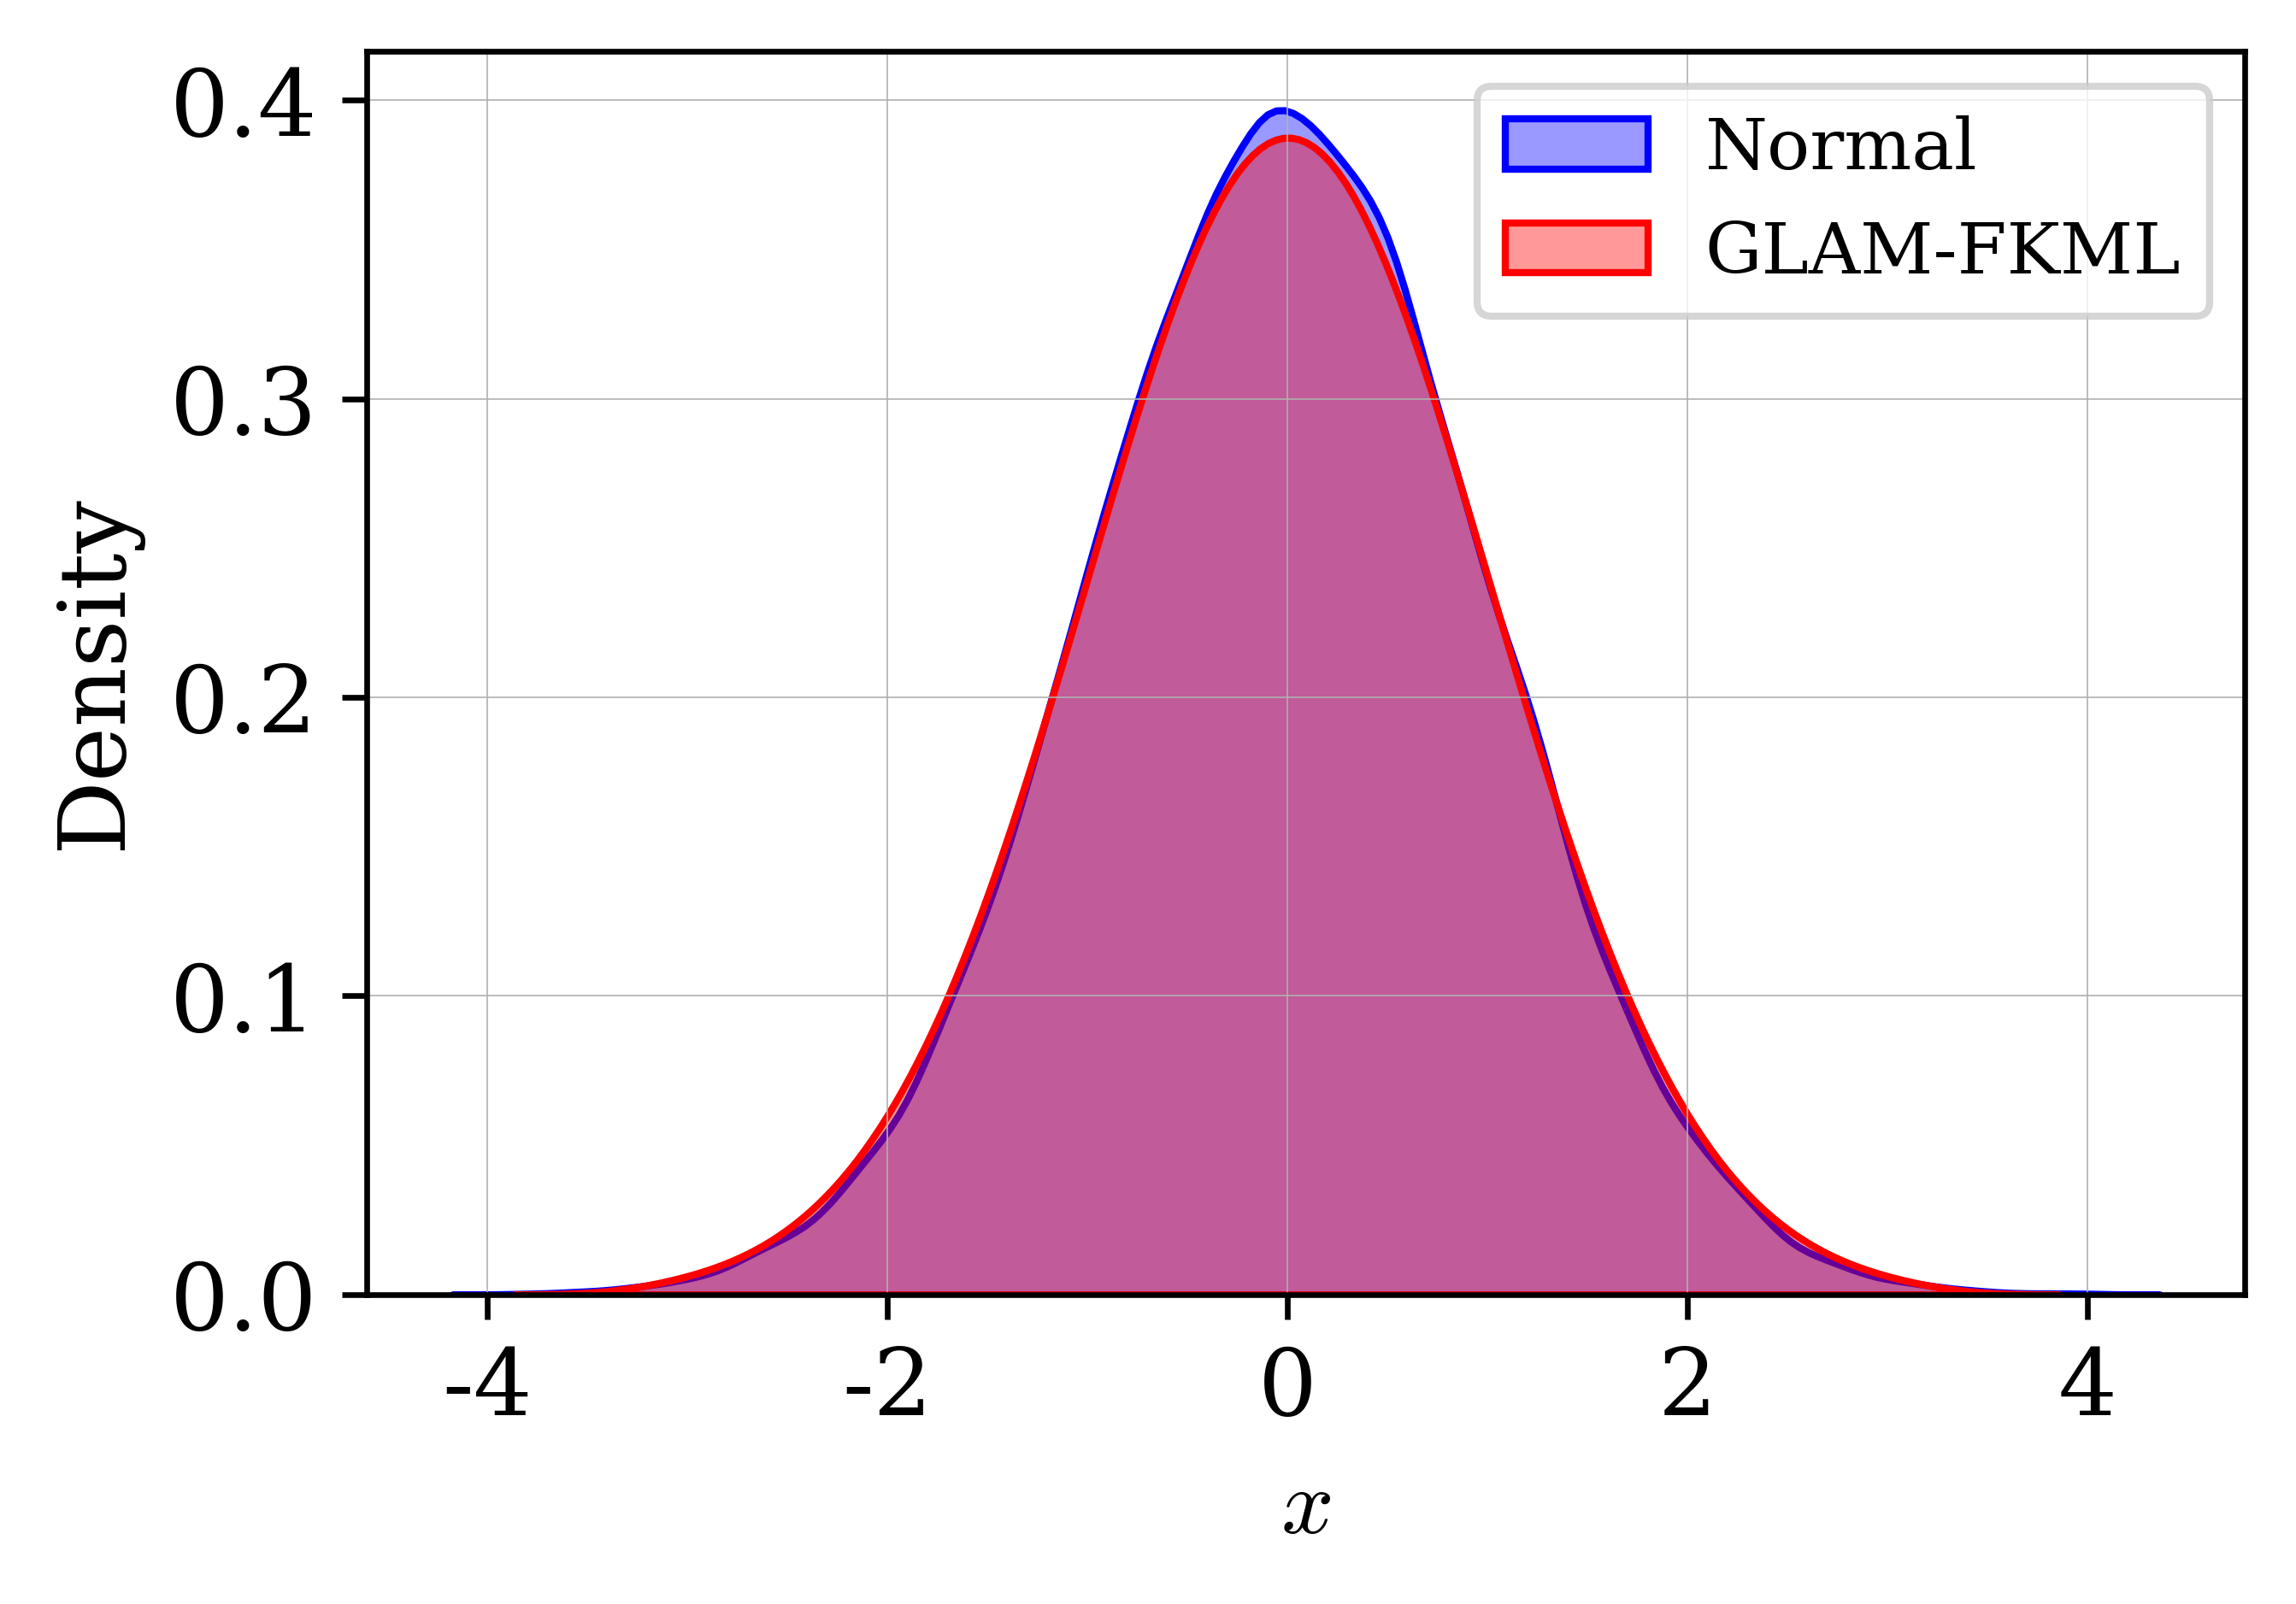
\includegraphics[width=\textwidth]{z_kde_histogram_compare.png}
        \caption{Normal}
        \label{fig:fit_normal}
    \end{subfigure}
    \hfill
    \begin{subfigure}[b]{0.32\textwidth}
        \centering
        
\includegraphics[width=\textwidth]{z_fig_gumbel.png}
        \caption{Gumbel}
        \label{fig:fit_gumbel}
    \end{subfigure}
    \hfill
    \begin{subfigure}[b]{0.32\textwidth}
        \centering
        
\includegraphics[width=\textwidth]{z_fig_uniform.png}
        \caption{Uniforme}
        \label{fig:fit_uniform}
    \end{subfigure}
    \vspace{0.2cm}
    \fonte{Autor (2025).}
\end{figure}

\subsection{Acoplamento com a Expansão em Caos Polinomial}

Seguindo a metodologia proposta por \textcite{ZhuSudret2021}, a GLD é acoplada à Expansão em Caos Polinomial (PCE) para a construção de um emulador global. Nesse arcabouço, a resposta estocástica do simulador para qualquer entrada $\mathbf{X}$ é modelada por uma GLD cujos parâmetros $\boldsymbol{\lambda}$ são, eles próprios, funções das variáveis de entrada.

Dado um conjunto de parâmetros de entrada $\mathbf{X}$ governado por uma função densidade de probabilidade conjunta $f_{\mathbf{X}}(\mathbf{x})$, cada componente do vetor de parâmetros $\lambda_i$ é aproximada por uma PCE truncada, conforme a Equação \eqref{eq:pce_lambda}:

\begin{equation}\label{eq:pce_lambda}
\lambda_i(\mathbf{X}) \approx \sum_{\boldsymbol{\alpha} \in \mathcal{A}} a_{i, \boldsymbol{\alpha}} \Psi_{\boldsymbol{\alpha}}(\mathbf{X}), \quad i = \{1, 2, 3, 4\}
\end{equation}

em que $\Psi_{\boldsymbol{\alpha}}(\mathbf{X})$ são polinômios ortonormais multivariados específicos das distribuições de entrada \cite{xiu2002}, $a_{i, \boldsymbol{\alpha}}$ são os coeficientes a determinar e $\mathcal{A}$ é o conjunto de multi-índices que define o esquema de truncamento, usualmente uma base de grau total \cite{blatman2011}.

Uma vez estimados os coeficientes, o emulador PCE--GLD fornece instantaneamente a distribuição de probabilidade completa, por meio dos parâmetros $\boldsymbol{\lambda}$, para qualquer nova entrada $\mathbf{X}^*$, sem exigir novas execuções do simulador estocástico original. Uma vantagem adicional do acoplamento com a PCE é que os índices de sensibilidade de Sobol podem ser obtidos analiticamente a partir dos coeficientes da expansão \cite{sudret2008}, permitindo quantificar, sem custo adicional, a contribuição de cada variável de entrada para a variância da resposta.

\subsection{Extensão ao Domínio Temporal}

O arcabouço PCE--GLD descrito nas seções anteriores é formulado para um instante fixo. Como o processo de carbonatação é inerentemente dependente do tempo, a aplicação pretendida nesta dissertação exige que a evolução da distribuição da margem de segurança seja capturada ao longo de toda a vida em serviço da estrutura. Propõe-se, para tanto, a extensão do arcabouço por meio de uma camada de regressão que recebe o tempo como variável de entrada contínua.

Nessa formulação, os parâmetros $\boldsymbol{\lambda}$ da GLD são avaliados em passos de tempo discretos e um modelo de aprendizado de máquina de múltiplas saídas --- a rede neural artificial descrita na \autoref{RNA} --- é subsequentemente treinado para mapear o espaço conjunto de variáveis físicas e tempo nos parâmetros da distribuição, atuando como interpolador contínuo entre os instantes efetivamente simulados. O procedimento concreto de construção desse emulador, incluindo o plano de experimentos, o número de réplicas e as métricas de validação adotadas, é detalhado no capítulo de metodologia.
